\section{Exigences typiques et considérations de conception}
Le sous-système de communications est un élément clé d'un satellite, car il est directement lié aux autres sous-systèmes, notamment :

- La charge utile (Payload) → Le sous-système de communication permet la transmission des données générées par la charge utile (ex : images, mesures scientifiques).

- Le sous-système de commande et de gestion des données (CDH - Command and Data Handling) → Il gère l’échange d’informations entre les différents sous-systèmes et assure la bonne exécution des commandes envoyées depuis la Terre.

- L’orbite du satellite → L’orbite détermine le temps de contact avec les stations terrestres, ce qui influence la capacité de transmission et réception des données.

- Le segment sol (stations terrestres) → Il permet de communiquer avec le satellite pour recevoir les données et envoyer des commandes.
\begin{figure}[H] % H force l'affichage ici
    \centering
    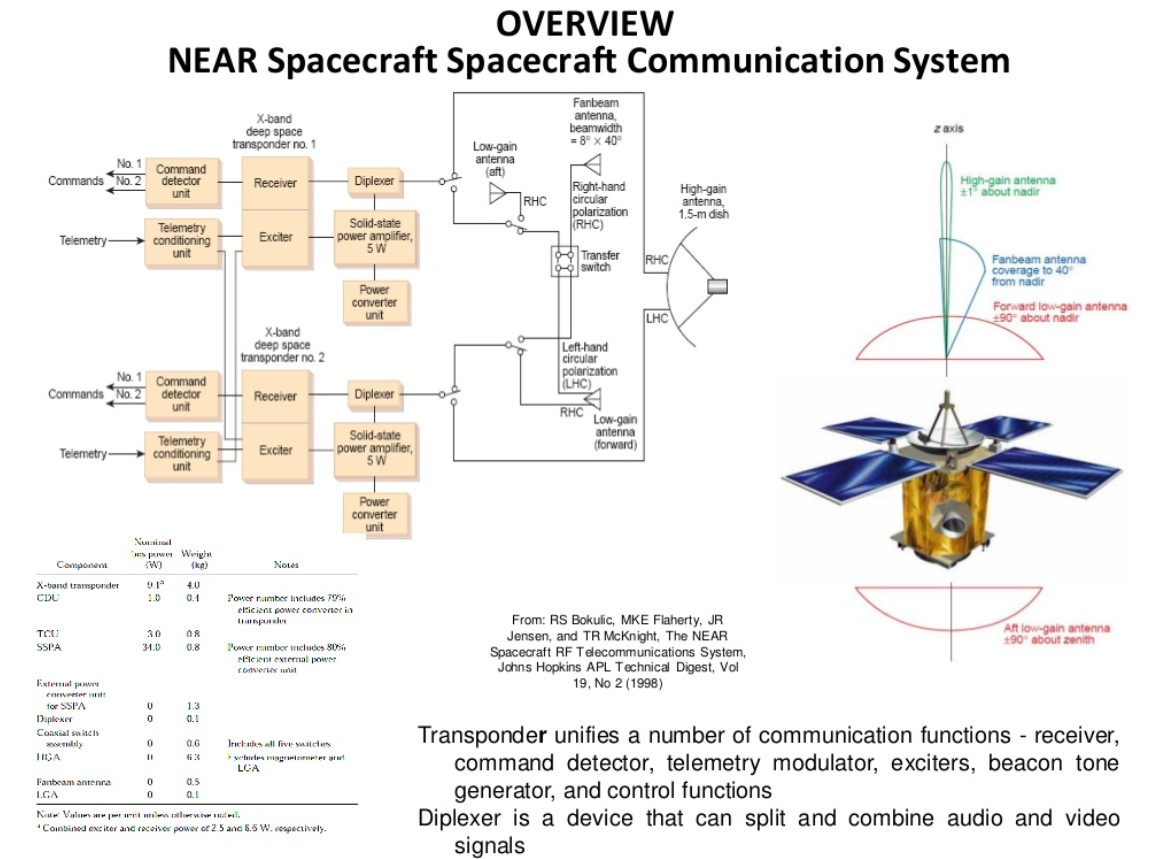
\includegraphics[width=0.8\textwidth]{figures/6-13.jpg}
    
    \caption{Présentation du système de communication du vaisseau spatial NEAR. Image de Pisacane.}
    \label{fig:communication2}
\end{figure}
Les \textbf{antennes} doivent être \textbf{dégagées de tout obstacle} pour assurer une bonne émission et réception des signaux. Elles peuvent être :
\begin{itemize}
    \item \textbf{Omnidirectionnelles} : émettant dans toutes les directions.
    \item \textbf{Directionnelles} : orientées vers une cible spécifique.
\end{itemize}
Les composants internes du sous-système de communication sont regroupés sur une \textbf{carte de communication} contenant :
\begin{itemize}
    \item \textbf{Amplificateurs} : Augmentent la puissance du signal.
    \item \textbf{Filtres} : Suppriment les interférences.
    \item \textbf{Diplexeurs} : Permettent d'utiliser une même antenne pour émettre et recevoir.
    \item \textbf{Récepteurs} : Captent les signaux venant du sol.
\end{itemize}
Cette carte est reliée à l’\textbf{ordinateur central} du satellite, contrôlé par le \textbf{sous-système de gestion des commandes et des données (CDH)}.Cette liaison permet:
\begin{itemize}
    \item \textbf{D'envoyer les commandes} depuis la Terre.
    \item \textbf{De transmettre les données} de la charge utile vers le sol.
\end{itemize}
Le traitement du signal peut se faire:
\begin{enumerate}[noitemsep, nolistsep]
    \item Directement sur la carte de communication, avec un traitement matériel dédié.
    \item Sur l’ordinateur central, offrant plus de flexibilité avec un traitement logiciel.
\end{enumerate}
Le sous-système de communication combine matériel et logiciel, reliant des antennes externes à une carte électronique dédiée, qui assure l'interface avec l’ordinateur central et le CDH.
\href{https://www.youtube.com/watch?v=NGgzq8eXZOQ&feature=youtu.be}{Deep Space Network: A Discussion on NASA’s Vital Lifeline to Spacecraft. Video by NASA/JPL}
\begin{itemize}[noitemsep, nolistsep]
    \item Responsabilités du spécialiste des communications du bus spatial :
    \begin{itemize}
        \item Il n'est pas responsable du segment sol.
        \item Il doit cependant coordonner avec le responsable du segment sol.
    \end{itemize}
     \item Contexte des réseaux de stations au sol :
    \begin{itemize}
        \item Les grandes agences (ex. NASA) disposent de réseaux comme le Deep Space Network :
        \begin{itemize}
            \item Couvre une large gamme de fréquences.
            \item Offre une couverture continue.
        \end{itemize}
        \item Les petits groupes (universités, entreprises) doivent :
        \begin{itemize}
            \item Construire leur propre réseau de stations au sol.
            \item Acheter un accès à un réseau existant.
        \end{itemize}
    \end{itemize}
    \item \textbf{Réseau SatNOGS :}
    \begin{itemize}
        \item Une \textbf{communauté ouverte} de stations au sol opérées par des passionnés.
        \item Implique des \textbf{opérateurs radioamateurs} du monde entier.
        \item Permet aux \textbf{petits satellites} d’envoyer des données, même sans accès au \textbf{Deep Space Network}.
    \end{itemize}
    \item \textbf{Accessibilité croissante des stations au sol :}
    \begin{itemize}
        \item Comme les engins spatiaux, leur construction et exploitation deviennent \textbf{de plus en plus accessibles}.
        \item Le mouvement \textbf{DIY} facilite leur développement pour les amateurs et passionnés.
    \end{itemize}
\end{itemize}
\begin{figure}[H] % H force l'affichage ici
    \centering
    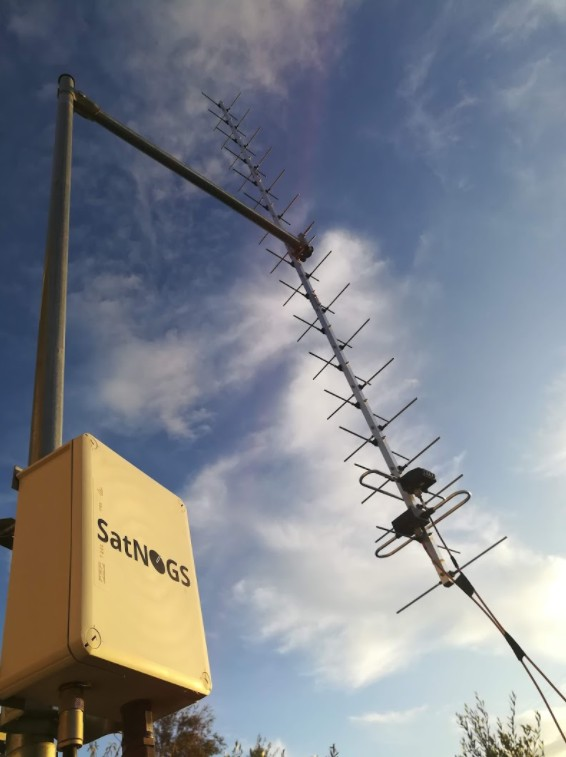
\includegraphics[width=0.8\textwidth]{figures/6-14.jpg}
        \caption{SatNOGS Network – Ground Station Avia. Image by Satnogs Network.}
    \label{fig:communication2}
\end{figure}
